% 05_results.tex — owned by this file: sec:results, tab:m2, tab:m3, tab:m4, tab:m5,
% fig:trajectory, fig:trajectory5m, fig:punishment, fig:ablation.
% Every number here is taken from paper/FACTS.md.

\section{Results: prices and the three behavioural tests}\label{sec:results}

This section reports the four pre-registered measurements of Section~\ref{sec:design}: the price level (M2), the reaction to a forced undercut (M3), the shortsightedness ablation (M4) and the unclaimed-temptation test (M5). Every cell has 100 seeds. $\Dl$ is measured on frozen greedy play after training; confidence intervals are mean $\pm\,1.96$ standard errors across seeds; ``high-price seeds'' are seeds with $\Dl > 0.5$. The pay-as-bid runs belong to Section~\ref{sec:phase1}.

\subsection{M2: price levels}

Table~\ref{tab:m2} gives $\Dl$ for the full learner and the two ablated learners at both horizons.

\begin{table}[htbp]
\centering
\caption{M2: collusion index $\Dl$ on frozen greedy play, 100 seeds per row. Notes: CI is the 95\% interval across seeds; ``converged'' means no firm's greedy action changed in the last 100,000 training rounds; the ablated learners are defined in Section~\ref{sec:learners}.}
\label{tab:m2}
\small
\setlength{\tabcolsep}{4pt}
\begin{tabular}{@{}llrrrrrr@{}}
\toprule
Learner & $T$ & $\Dl$ mean & 95\% CI & Median & Min--max & Seeds $\Dl>0.5$ & Converged \\
\midrule
Full ($\gamma=0.95$, $m=1$) & 1M & 0.375 & 0.354--0.397 & 0.343 & 0.143--0.679 & 12\% & 0\% \\
Full ($\gamma=0.95$, $m=1$) & 5M & 0.621 & 0.612--0.630 & 0.625 & 0.518--0.714 & 100\% & 100\% \\
$\gamma=0$, $m=1$ & 1M & 0.373 & 0.353--0.393 & 0.386 & 0.071--0.619 & 5\% & 0\% \\
$\gamma=0$, $m=1$ & 5M & 0.370 & 0.350--0.390 & 0.386 & 0.071--0.619 & 4\% & 100\% \\
$\gamma=0.95$, $m=0$ & 1M & 0.943 & 0.931--0.955 & 0.929 & 0.714--1.000 & 100\% & 79\% \\
$\gamma=0.95$, $m=0$ & 5M & 0.943 & 0.931--0.954 & 0.929 & 0.714--1.000 & 100\% & 100\% \\
\bottomrule
\end{tabular}
\end{table}

\paragraph{At the pre-registered horizon nothing has converged.}
At the specified horizon the full learner reaches $\Dl = 0.375$ (CI 0.354--0.397), a mean frozen clearing price of \eur{43.8}/MWh, and no seed has converged. The spread is wide: 1 seed below 0.2, 85 between 0.2 and 0.5, and 14 at or above 0.5 (12 strictly above).
% TODO-FACT: FACTS.md gives "14 in [0.5,0.7)" and "12% with Δ>0.5" separately; the 2 seeds at exactly Δ = 0.5 (price €55.00) should be entered in FACTS.md §3.
Figure~\ref{fig:trajectory} shows the process still moving. The mean price falls to about \eur{40} early in the run, while $\varepsilon_t$ is still large, and then drifts up; a few seeds jump to a higher band before the horizon. We read the early fall as the learners finding the undercut, but this section does not test that reading.
% TODO-FACT: round at which the mean price first reaches €40 and the timing of the late jumps are not in FACTS.md.

\begin{figure}[htbp]
\centering

\includegraphics[width=\textwidth]{figures/price_trajectory.png}
\caption{Mean clearing price per 1,000 rounds during training, full learner, 1M rounds. Thin lines are the 100 seeds; the thick line is their mean. Dashed lines mark the competitive (\eur{10}) and collusive (\eur{100}) benchmarks.}
% TODO-FACT: block length of the trajectory figures (collusim.agents.BLOCK) is not in FACTS.md; enter the figure script's settings there.
\label{fig:trajectory}
\end{figure}

Five million rounds finish the process (Figure~\ref{fig:trajectory5m}). Seeds leave the \eur{40} band one at a time, jump to a mean price between \eur{60} and \eur{72}, and never move again. Every seed converges; the round of the last change in any firm's greedy action has median 1.63M (range 1.20M--2.88M).
% TODO-FACT: confirm this is how the convergence round is defined in results/*.json.
All land in a narrow band: $\Dl = 0.621$ (CI 0.612--0.630), 99 seeds in $[0.5, 0.7)$ and one above, mean frozen price \eur{65.9}/MWh. The acceptance criterion for M2 fails at the pre-registered 1M horizon and is met at 5M, a horizon added after the 1M result was seen and not itself pre-registered (Section~\ref{sec:design}). The M2 criterion was written as `a meaningful fraction of seeds above $\Dl = 0.5$' without a number; we read 12\% at 1M as failing it and 100\% at 5M as meeting it, and a reader who counts 12\% as meaningful should treat M2 as met at both horizons.
% TODO-FACT: the pre-registered wording of the M2 rule.
The ablated learners converge sooner: median 1.26M rounds (1.14M--1.45M) for $\gamma = 0$ and 0.83M (0.72M--0.99M) for memory 0.

\begin{figure}[htbp]
\centering
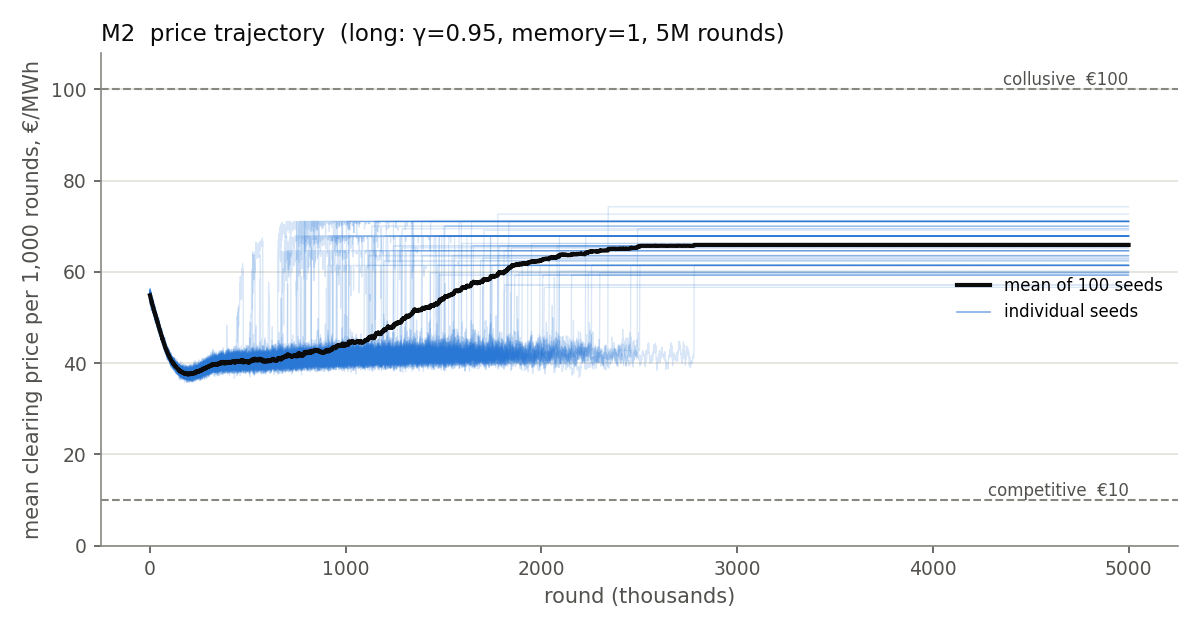
\includegraphics[width=\textwidth]{figures/price_trajectory_long.png}
\caption{As Figure~\ref{fig:trajectory}, for 5M rounds. Seeds jump one at a time from the \eur{40} band to \eur{60}--\eur{72} between roughly 1.2M and 2.9M rounds and then stay there.}
\label{fig:trajectory5m}
\end{figure}

\paragraph{What the converged policies do.}
The converged full learners do not sit at a constant high price. Reading the frozen state sequence, 86 of 100 seeds play a cycle of period four or less (period 1: 3 seeds; 2: 35; 3: 21; 4: 27); the rest run 5-, 6- or 7-cycles (7, 5 and 2 seeds). The 35 two-cycles alternate a near-symmetric high profile, bids \eur{94}--\eur{100} with mean high price \eur{96.5}, and a near-symmetric low profile, bids \eur{36}--\eur{42} with mean low price \eur{41.0}. Bid profiles are quoted rounded to the euro; the rungs are $10, 16.43, \dots, 93.57, 100$ (Section~\ref{sec:market}). One example is a seed that bids $(100, 94, 100)$ in round $t$, clearing at \eur{100}, then $(36, 42, 36)$ in round $t+1$, clearing at \eur{36}, and repeats. The most common last-round profiles are $(100,100,100)$ in 13 seeds and $(94,94,94)$ and $(36,42,42)$ in 6 each. At 1M rounds, before convergence, periods range from 1 to 56 and only 23 seeds have period four or less.

The $\gamma = 0$ learner converges to long, irregular cycles (20 of 100 seeds with period four or less, periods up to 25) whose most common last-round profiles have one firm at cost: $(10,16,16)$ in 15 seeds, $(10,36,36)$ and $(10,42,42)$ in 10 each.

The memory-0 learner converges at 5M rounds, in all 100 seeds, to a fixed point of the form (low, high, high): one firm bids low and the other two tie high. The low bidder sits at \eur{10} in 36 seeds, \eur{16.43} in 31, \eur{22.86} in 18, \eur{29.29} in 11, and \eur{42.14} or \eur{67.86} in 2 each; the high pair sits at the cap in 43 seeds, at \eur{93.57} in 36, at \eur{87.14} in 20 and at \eur{74.29} in 1. The most common profile, $(10,100,100)$, appears in 21 seeds. Because the clearing price is the second-lowest bid, it equals the high bid; the low bidder sells 60 MW at that price and earns the most, and each high bidder sells 20 MW. The mean frozen price is \eur{94.9}/MWh, $\Dl = 0.943$. None of these fixed points is a one-shot Nash equilibrium of Table~\ref{tab:nash}: at $(22.86, 100, 100)$, for example, each high bidder earns \eur{1{,}800} per round and could earn \eur{3{,}343} by bidding \eur{93.57}. Section~\ref{sec:phase1} returns to this.

\subsection{M3: punishment}

The punishment test adapts the impulse-response design of \citet{calvano2020}. With learning frozen, greedy play settles for 200 rounds, six pre-deviation rounds are recorded, one firm is forced to bid \eur{10} for a single round, and 24 rounds of greedy play follow. The verdict is read from the rivals' bids against a counterfactual path with no deviation, so that a converged cycle is not mistaken for a reaction, in two 12-round windows (12 divides the cycle lengths 1--4 and 6). ``Punish-forgive'': rivals at least half a rung (\eur{3.21}) below the counterfactual in rounds 1--12 and back within half a rung in rounds 13--24. ``Punish, no recovery'': below in both windows. ``No reaction'': rivals' bids do not move. Table~\ref{tab:m3} reports the verdicts with firm 1 as the deviator.

\begin{table}[htbp]
\centering
\caption{M3: verdicts of the punishment test, deviator firm 1. Notes: ``no-op'' counts seeds in which the deviator was already bidding \eur{10}, so the forced deviation changed nothing; those seeds are still judged. A no-op is ``no reaction'' by construction, since the forced bid equals the counterfactual; the no-op share is therefore part of the no-reaction share. Seed counts are in parentheses for the rows with fewer than 100 seeds. The last column counts seeds with a punish-forgive verdict for at least one of the three possible deviators.}
% TODO-FACT: the parenthesised counts are percentage × seeds judged (e.g. 33% of 12 = 4); confirm against results/indicators_*.json and enter the counts in FACTS.md §4.
\label{tab:m3}
\footnotesize
\setlength{\tabcolsep}{3pt}
\begin{tabular}{@{}llrrrrrr@{}}
\toprule
 & & & Punish-- & Punish, & No & & Forgive, \\
Learner & $T$ & Seeds & forgive & no recovery & reaction & No-op & $\geq 1$ deviator \\
\midrule
Full ($\gamma=0.95$, $m=1$) & 1M & 12 ($\Dl>0.5$) & 33\% (4) & 50\% (6) & 17\% (2) & 8\% (1) & 67\% (8) \\
Full ($\gamma=0.95$, $m=1$) & 5M & 100 (all) & 21\% & 70\% & 9\% & 2\% & 47\% \\
$\gamma=0$, $m=1$ & 1M & 5 ($\Dl>0.5$) & 0\% (0) & 20\% (1) & 80\% (4) & 40\% (2) & 40\% (2) \\
$\gamma=0$, $m=1$ & 5M & 4 ($\Dl>0.5$) & 25\% (1) & 25\% (1) & 50\% (2) & 25\% (1) & 50\% (2) \\
$\gamma=0.95$, $m=0$ & 1M / 5M & 100 (all) & 0\% & 0\% & 100\% & 10\% / 11\% & 0\% \\
\bottomrule
\end{tabular}
\end{table}

\begin{figure}[htbp]
\centering

\includegraphics[width=\textwidth]{figures/punishment_long.png}
\caption{M3 in the 5M full-learner runs. Left: bids and clearing price around the forced deviation for the seed with the highest $\Dl$ (the figure's agents 0, 1, 2 are firms 1, 2, 3). Right: mean clearing price across all 100 seeds, with the no-deviation counterfactual dotted.}
% TODO-FACT: which seed the left panel shows is not in FACTS.md; enter the figure script's seed selection there. When figures/punishment_long.png is regenerated, relabel its legend "firm 1/2/3" and delete the parenthetical (appendix.tex carries the canonical 0,1,2 mapping).
\label{fig:punishment}
\end{figure}

\paragraph{Reading.}
In the converged 5M runs a deviation is answered in 91\% of seeds. Over all 100 seeds the rivals' bids over rounds 1--12 average \eur{16.7} below the counterfactual, and the mean clearing price falls from \eur{66.0} to \eur{45.1} against a counterfactual of \eur{65.9}. The second window splits the 91\%. In 21\% the rivals are back by rounds 13--24: their drop shrinks from \eur{10.9} to \eur{0.2} and the price in that window is \eur{63.2} against \eur{65.4}. That is the punish-then-forgive pattern. In 70\% the rivals drop \eur{20.5} and are still \eur{19.1} below in the second window; the price stays at \eur{41.8} and then \eur{43.8} against \eur{66.2}. The test does not say whether this is a learned response to the deviation or the absence of any learned route back to the cycle; Section~\ref{sec:residual} bears on that question. In 9\% the rivals never move. Nine of the 100 long-run seeds play 5- or 7-cycles, which the 12-round windows do not cover; their verdicts can be misread, and the forgive/no-recovery split should be read with that in mind (Section~\ref{sec:discussion}).

Changing the deviator gives the same split in aggregate (firm 2: 20 forgive, 69 no recovery, 11 none; firm 3: 17, 73, 10), but the verdict for a given seed changes with the deviator in 61 of 100 seeds. The verdict is therefore a property of the seed and the deviator together, not of the seed alone. Part of this is mechanical: at the asymmetric profiles many seeds converge to, forcing a different firm to \eur{10} is a different deviation. The memory-0 control behaves as it must: with a single state there is nothing to react to, and 100\% of seeds show no reaction. The test therefore reads differently on the two learners, but for a reason that has nothing to do with strategy: a one-state table cannot react to anything, so the test detects the state definition, not a learned continuation (Section~\ref{sec:discussion}). The memory-1 learner passes its weak form (rivals react) in 91\% of seeds and its full form (react, then forgive) in 21\%.

From a profile at which the two lowest bids are tied, which includes the symmetric profiles the full learner converges to, the one-round deviation is profitable for the deviator and leaves the clearing price unchanged, because the price is the second-lowest bid; from an asymmetric profile, such as the memory-0 rest point, it can move the price and need not be profitable (Section~\ref{sec:market}). Section~\ref{sec:phase1} uses this.

\subsection{M4: shortsightedness ablation}

The ablation asks whether the high price needs memory of the past or a value on the future. The collapse criterion was fixed in advance: an ablated learner has collapsed if its $\Dl$ is below 0.25 and below half the full learner's $\Dl$. Table~\ref{tab:m4} and Figure~\ref{fig:ablation} give the outcome.

\begin{table}[htbp]
\centering
\caption{M4: collusion index of the full learner and the two ablated learners, with the pre-registered verdict. Notes: collapse requires $\Dl < 0.25$ and $\Dl$ below half the full learner's value.}
\label{tab:m4}
\begin{tabular}{lrrrl}
\toprule
$T$ & Full learner & $\gamma=0$ & Memory 0 & Verdict \\
\midrule
1M & 0.375 & 0.373 (not collapsed) & 0.943 (not collapsed) & fail \\
5M & 0.621 & 0.370 (not collapsed) & 0.943 (not collapsed) & fail \\
\bottomrule
\end{tabular}
\end{table}

\begin{figure}[htbp]
\centering

\includegraphics[width=\textwidth]{figures/ablation_bars.png}
\caption{M4 ablation at 1M rounds (left) and 5M rounds (right). Bars are the mean $\Dl$ across 100 seeds, whiskers the 95\% CI, dots the individual seeds.}
\label{fig:ablation}
\end{figure}

The test fails at both horizons. Removing the future ($\gamma = 0$) leaves $\Dl$ at 0.373 at 1M and 0.370 at 5M. At the specified horizon, where neither learner has converged, this is statistically indistinguishable from the full learner (0.375 against 0.373). At 5M the myopic learner does sit lower, 0.370 against 0.621: setting $\gamma = 0$ removes about 40\% of the converged price premium, not all of it, and 0.370 is far from collapse. Removing the past does the opposite of what the criterion anticipates: the memory-0 price rises to $\Dl = 0.943$ at both horizons. By the specification's own rule the M2 result cannot be attributed to tacit collusion on this evidence. The two ablated learners reach their prices by different routes, long irregular cycles in one case and an asymmetric fixed point in the other, but the ablation compares only $\Dl$ and cannot tell them apart.

\subsection{M5: unclaimed temptation}

At every state on the cycle of frozen play (the converged cycle at 5M; at 1M, the cycle of the frozen but unconverged table, Section~\ref{sec:indicators}), for each firm, the test computes the best one-shot deviation profit minus the realised profit, rivals held fixed. The verdict is ``unclaimed temptation'' if any gap is positive and ``static Nash'' if all gaps are zero.

\begin{table}[htbp]
\centering
\caption{M5: seeds with a profitable, unplayed one-shot deviation on the cycle of frozen play, and the mean best gap per round over seeds with $\Dl > 0.5$.}
\label{tab:m5}
\small
\begin{tabular}{@{}lrr@{}}
\toprule
Configuration & Seeds with unclaimed temptation & Mean best gap (\eur{}/round) \\
\midrule
Full ($\gamma=0.95$, $m=1$), 1M, $\Dl>0.5$ & 100\% (100\% of all seeds) & 2,475 \\
Full ($\gamma=0.95$, $m=1$), 5M & 100\% & 2,226 \\
$\gamma=0$, 1M / 5M & 100\% of $\Dl>0.5$ (95\% of all seeds) & 1,209 / 1,221 \\
Memory 0, 1M / 5M (control) & 100\% & 1,444 / 1,448 \\
\bottomrule
\end{tabular}
\end{table}

The temptation is large and, outside the 5\% of $\gamma = 0$ seeds that end at one-shot Nash profiles, present in every seed (Table~\ref{tab:m5}). At the all-cap profile each firm earns \eur{3{,}000} per round and could earn \eur{5{,}400} by shaving one rung off its bid: the price would not move and the firm would sell its full 60 MW. Nobody does. Read on its own, and only for the memory-1 learner, this is what the literature treats as the fingerprint of anticipated retaliation, and M3 would appear to agree. But the memory-0 control leaves the same kind of money on the table in 100\% of seeds, a mean gap of \eur{1{,}444} to \eur{1{,}448} per round, while being structurally incapable of anticipating anything. The 5\% of $\gamma = 0$ seeds without temptation sit at one-shot Nash profiles such as $(10,16,16)$. In this market the fingerprint is produced by a learner with no memory as readily as by one with memory, so on its own it is not discriminating.

\paragraph{Summary of verdicts.}
M2 fails at the pre-registered horizon and is met only at the 5M horizon added afterwards. M3 is partial: rivals react to a forced undercut in 91\% of converged seeds and forgive within 24 rounds in 21\%, and the memory-0 control shows no reaction in any seed. M4 fails at both horizons: neither ablation collapses the price, and the memory-0 learner prices higher than the full learner. The M5 fingerprint is present in 100\% of seeds, but equally in the memory-0 control. The learners converge to supra-competitive prices under these parameters, and the standard indicators do not support calling the outcome tacit collusion; none of the three behavioural tests separates a learner that has learned a continuation from one that carries a stale estimate; M3 reads differently on the two learners only because a one-state table has nothing to react to. Section~\ref{sec:phase1} asks what does, and Section~\ref{sec:discussion} collects the verdicts in Table~\ref{tab:indicators-summary}.
